\subsection{Pièces interchangeables et réparable : la technologie du futur ? }

Dans la partie \ref{c1/s1/ss1:preuve_op}, nous citions l'exemple des iPods d'apple, dont la batterie était collée. Lorsque celle-ci tombait en panne,  l'appareil entier était à changer. 
Cet exemple est loin d'être un cas à part. N'importe quel ordinateur portable est soumis à cette obsolescence fonctionnelle. Lorsque la carte mère d'un PC rend l'âme, il est quasiment impossible de réparer l'ordinateur. Pourtant, la pièce responsable de la panne est seulement un support sur laquelle sont implanté d'autres composants, qui restent fonctionnel après la mort de la carte mère.  

Pourtant, dans le monde des ordinateurs fixe, une solution existe qui permet de contourner l'obsolescence fonctionnelle : monter soit même son pc. Chaque pièce, choisi par l'utilisateur, est amovible. En cas de panne, prenons l'exemple de la carte graphique, il est facile de remplacer la pièce abimée. Ainsi, l'\op peut être réduite par cette manière. 


Cette idée peut elle être étendue ? 

\bigbreak

Cette idée arrivera peut-être dans le monde du smartphone. En 2013, Dave Hakkens lance l'idée d'un téléphone modulable. Chaque pièce peut être changée au goût de l'utilisateur. Depuis la sortie de ce projet, de nombreux concurrents ont vu le jour : Google développe le projet Ara,  l'entreprise finlandaise \textit{Circular Devices OY} a dévoilé en décembre 2014 son projet de smartphone modulaire : le Puzzlephone. Les trois projets sont censés arriver sur le marché durant l'année 2015, cependant, aucune date officielle n'a encore été fixée. Il reste fort probable qu'un smartphone modulable sortira dans les prochaines années. 
\medbreak
Une autre solution consisterait à réparer les pièces abimées.  L'émergence des imprimantes 3D et des fab lab pourrait fortement aider  à faciliter à dépanner les objets actuels cassés. 

\begin{wrapfigure}{l}{0.3\linewidth}\begin{center}
\vspace{-0.7cm}
\includegraphics[scale=0.33]{Rsc/logofablab.jpg} 

\textit{Logo officiel des fablabs}
\end{center}
\end{wrapfigure}

Un fablab (contraction de fabrication laboratory : laboratoire de fabrication) est un espace ouvert au public où l'utilisateur peut avoir accès à )à toute sorte d'outil pour réaliser des objets. Ainsi le fab lab de Rennes met à disposition du public une imprimante 3D, et propose également des initiations à la programmation sur carte Arduino. 
Ces deux éléments peuvent être très utile pour luter contre l'\op. 

L'imprimante 3D est un outil programmable par ordinateur qui permet de fabriquer n'importe quel objet en plastique. Imaginons qu'une personne lambda casse une pièce plastique d'un parapluie. Pour réparer son produit, il lui suffira de recréer cette pièce via une fab lab (ou une imprimante 3D personnelle, on en trouve désormais à moins de 1000\euro. Il peut être facilement imaginé que les plans de la pièce soit mis sur internet. 

\begin{wrapfigure}{r}{0.3\textwidth}
\begin{center}
\vspace{-1cm}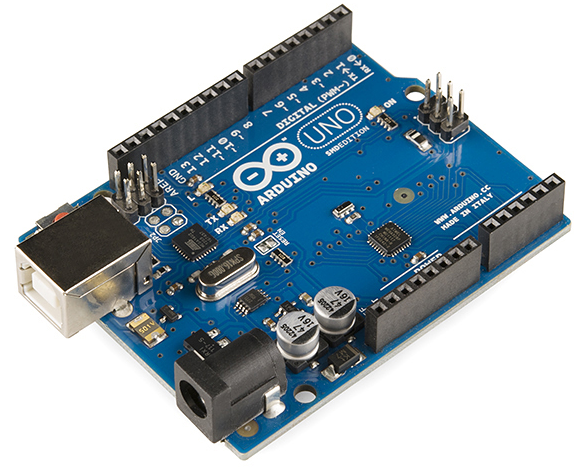
\includegraphics[scale=0.25]{Rsc/Arduino.png} 

\textit{Une carte Arduino}
\end{center}
\end{wrapfigure}

Une carte Arduino est une carte électronique qui se veut accessible à tous. Elle est relativement peu coûteuse, entre 30 et 50\euro~ selon les modèles. Basée sur une version simplifiée du langage C, elle est facilement programmable. Comme elle est très populaire, de nombreux tutoriels existent sur internet. Les débutants ont donc de nombreuses manières d'apprendre à utiliser cette carte. Elle pourrait être utilisé pour réparer un sèche linge défectueux, en reprogrammant la pièce cassée.

\medbreak

Suite à la volonté du gouvernement français de développer les fablabs, leur nombre est en pleine extension. En 2013, la ministre déléguée chargée des PME Fleur Pellerin lance un appel à projet pour subventionner et développer les fablabs sur le territoire français. Près de 150 réponse auront étés présentées. 15 parmi celle ci ont été retenues. Ainsi,  ce type d'organisation est amené a être de plus en plus présente dans nos vies. 

La monographie \textit{Fablabs et imprimantes 3D}, rédigée par cinq étudiants de l'INSA de Rennes en 2013, contient une partie entière sur la possibilité de lute contre l'\op. Nous vous invitons à consulter leur site web pour plus d'information\footnote{\url{http://diy-fablab.insa-rennes.fr}}.


\bigbreak 

Ces idées sont certes prometteuse, mais elle nous semblent difficilement applicable. L'exemple du Phonebloks est flagrant : malgré un plébiscite de près d'un million de consommateur, le smartphone n'est toujours pas sorti. Leur principale difficulté est de trouver des industriels acceptant de travailler avec eux. C'était d'ailleurs le but de la vidéo promulguée sur youtube \cite{pb_yt} : faire du bruit (\textit{thunderclap}) afin de convaincre les industriels d'accepter de collaborer avec Phonebloks. Si une quinzaine d'entreprise sont partenaire du projet, il est à noter l'absence de producteurs de processeur. 


\medbreak
Réparer les pièces semble également être compromis, du moins dans le domaine électronique. En effet, les composants électroniques sont de nos jours microscopique. Les consommateurs sont en effet demandeurs de produits toujours plus performant. Il est difficile d'imaginer un téléphone portable sans GPS ni bluetooth, alors que c'était la norme il y a dix ans. Pour satisfaire ce désir, les fabricants ont réduit la taille des composants de base. 

Le soudage a aussi été abandonné. Auparavant, pour fixer les éléments électroniques, on les soudait : une broche était passée au travers de la carte électronique, puis fixée grâce à de l'étain. Cette technologie possédait l'avantage d'être réversible : il est facile d'enlever un composant défectueux et de le remplacer. 

La technique actuelle, qui permet la miniaturisation, est appelée le Composant Monté en Surface (CMS). Au lieu d'être soudé, le composant est brasé (comprendre collé) à la carte mère. Le CMS est bien plus avantageux que les anciennes techniques : le temps de fabrication est réduit (pas de perçage de la plaque, plus facilement automatisable) le poids et la taille  sont réduit. Cette technologie a naturellement été choisie par les industriels ; elle répond aux exigence de coup, de taille et de poids des consommateurs. Le principale inconvénient de cette méthode est la maintenance : réussir a identifier la pièce responsable du dysfonctionnement est largement compliqué par la miniaturisation (il faut penser que la taille d'une resistance de type CMS est de  l'ordre du millimètre) ; réussir à extraire la pièce coupable sans abimer le reste de la carte devient extrêmement ardu. 

Pour pouvoir  réparer facilement un produit, il faudrait donc pouvoir réutiliser des techniques de soudage. Ceci est difficilement réalisable car : 
\begin{itemize}
\item le produit serait 10 fois plus gros : la taille d'une résistance CMS est de l'ordre du millimètre, celle d'une résistance à souder est de l'ordre du centimètre ;
\item le produit serait plus cher. 
\end{itemize}
Le consommateur serait il prêt à payer plus cher pour un produit plus gros ? C'est peu probable.

\medbreak

Certains espèrent réparer les produits avec une carte Arduino. Sur ce point aussi nous sommes sceptique. 

Comme nous l'avons expliqué précédemment, il est difficile de remplacé un composant issu de la miniaturisation. Il est donc nécessaire de remplacer une grande partie du produit pour réparer la pièce cassée. La tâche semble possible ; malgré tout, il faudra comprendre le fonctionnement de la partie à remplacer par sois même (les constructeurs ne donnent pas en libre source les plans de leur inventions), puis réussir à reprogrammer cette partie. Cette tache est donc un travail de longue haleine. 

Il est possible que, comme dans le domaine de l'informatique, des implémentations libres soient téléchargeable sur internet : un utilisateur développe une solution dépannant le sèche linge dont nous prenions l'exemple plus tôt. Il mettrait ensuite le code source en libre service sur internet. Mais a-t-il le droit de le faire ? 

\medbreak 

Une partie tout à fait réalisable est le remplacement de pièce plastique. En effet, le bouton que nous souhaitions réparer est beaucoup plus gros que les carte électroniques. Il est possible d'observer la pièce et de la reproduire sur ordinateur pour ensuite l'imprimer. De plus, on peut imaginer le même principe de distribution sur internet du plan. Dans ce cas, la question légale se pose : la législation française autorise-t-elle cette pratique. 

\bigbreak

Ainsi, les Fablabs constituent une solution pour luter contre l'\op. Cependant, le projet semble quelque peu idéaliste par rapport au souhait des consommateurs actuels. 
\bigbreak

